%
% File: chap01.tex
% Author: Joshua Carey

%
\let\textcircled=\pgftextcircled\chapter{Background}\label{chap:background}

% \initial{T}his chapter delves into the application of machine learning in sailboat control, with a particular emphasis on utilising kites as a means of propulsion. The exploration of kite-powered vessel technologies presents a novel avenue to enhance the efficiency of sailboats. The fusion of machine learning, specifically Reinforcement Learning (RL), with kite propulsion systems, opens up a realm of possibilities for autonomous sailboat control. 



% The subsequent sections will provide an in-depth examination of kite-powered vessel technologies, introduce the core concepts of RL, discuss relevant literature, identify gaps in current research, and highlight the novelty and potential contributions of the proposed work. 

% \initial{T}he maritime domain has long been a focal point of innovation and technological advancement. Historically, propulsion mechanisms have evolved from rudimentary oars to sophisticated sails, each iteration seeking to harness nature's forces more efficiently. Today, as we stand at the intersection of technology and tradition, there emerges a compelling avenue for exploration: kite-powered vessels. This innovative approach to propulsion seeks to leverage the aerodynamic advantages of kites, offering potential enhancements in efficiency and menoeuverability over traditional sails.

\initial{M}aritime innovation has consistently driven technology forward, transitioning from simple oars to advanced sails. With the emergence of highly efficient and mass produced recreational kites, kite-powered vessels are at the forefront of maritime innovation, aiming to outperform traditional sails in efficiency, manoeuvrability and reliability.

However, the introduction of kites as a propulsion mechanism brings forth a new set of challenges. The dynamic nature of kites, combined with the unpredictable marine environment, requires advanced control systems capable of real-time adaptation and decision-making, in order to be a viable replacement for sails. This is where the application of machine learning, and more specifically Reinforcement Learning (RL), becomes paramount. An RL agent learns to make decisions that maximise a certain objective, often framed as a cumulative reward. The potential of RL in maritime propulsion is evident: it offers a framework for developing control systems that can adapt to changing conditions, environments and learn from experience. 

This chapter aims to provide an in depth background into the technologies that will be leveraged in this thesis. This includes a detailed examination of the core concepts of RL, the mechanisms behind the PPO algorithm, and the Unity game engine. We will also explore the current state of kite-powered vessel technologies, identify gaps in existing research, and highlight the novelty and potential contributions of the proposed work.

\section{Reinforcement Learning (RL)}\label{RL_background}
% User
% Write me a technical and informative introduction for Reinforcement Learning (RL). This is part of the background section of a thesis and will lay the foundation for how and why RL can/has/might want to be used to control boats (and kites instead of sails). Make it about 1000 words and include citations for your sources. The style should be informative but upbeat. 

Reinforcement Learning (RL) is a prime example of machine learning and has been a hot topic in artificial intelligence (AI) over the last few years, with applications ranging from autonomous driving to sophisticated game-playing algorithms. At its core, RL is about learning by interaction: an agent takes actions in an environment to maximise some notion of cumulative reward. The agent learns from the consequences of its actions, rather than from being explicitly taught, making it a powerful tool for tasks where the optimal strategy is unknown or hard to define$~$\cite{sutton2018reinforcement}.

Imagine teaching a child to ride a bicycle. You don't provide a step-by-step manual; instead, the child learns by trying different actions (like pedaling or balancing) and receiving feedback (falling down or moving forward). This trial-and-error approach is the essence of how RL works. The agent (in this case, the child) interacts with its environment (the bicycle and the ground) and learns a policy that dictates the best action to take in any given situation based on the rewards (or penalties) it receives$~$\cite{watkins1992qlearning}. Figure$~$\ref{fig:rl_diagram} illustrates this loop.

\begin{figure}
    \centering
    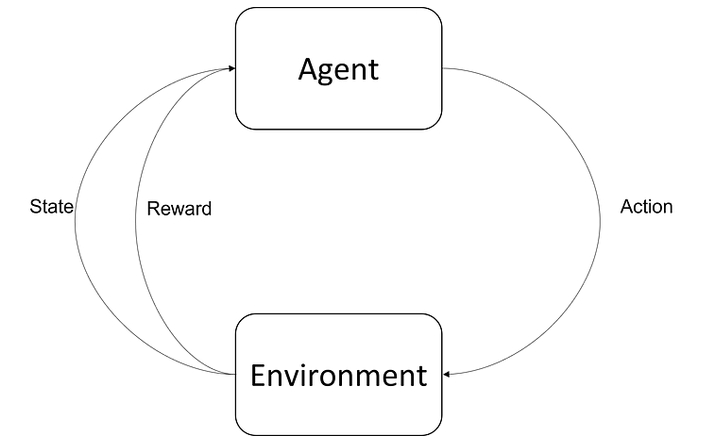
\includegraphics[width=0.8\textwidth]{Images/RL_Loop.png}
    \caption{A diagram of the RL Loop}\label{fig:rl_diagram}
\end{figure}

Historically, RL has its roots in the fields of operations research and behavioral psychology. The idea of learning optimal strategies through interaction has been explored in various contexts, from game playing to industrial optimisation$~$\cite{bellman1957dynamic} to fine-tuning large language models as recently shown by OpenAI. However, it's the modern advancements in computational power and algorithms, of the last few years, that have propelled RL to the forefront of AI research. Games like Go, which were once considered too complex for computers to master, have now been conquered by RL agents, showcasing the potential of this approach\cite{silver2016mastering}.

Boats, with their intricate dynamics and the unpredictable nature of water, present a challenging environment for control systems. Traditional control methods often rely on predefined rules and heuristics, which might not always be optimal or apply to unique situations, especially in changing conditions. These autonomous controls vary from something as simple as a piece of bungee to Proportional–integral–derivative (PID) controllers to more complex systems like Model Predictive Control (MPC)$~$\cite{erhard2013control}. Enter RL. With its ability to learn from experience, an RL-based control system should be able to adapt to varying conditions, ensuring smooth sailing even in turbulent waters, and gusty winds.

But why stop at boats? The concept of using kites to harness wind power for propulsion is not new. Historically, kites have been used in various cultures for fishing, transportation, and even warfare$~$\cite{hallion2003taking}. In the modern context, kites offer an exciting alternative to traditional sails, providing more power and manoeuvrability. However, controlling a kite, especially in varying wind conditions, is a complex task.  Kite control has only been explored in recent years, primarily in the field of renewable energy, where large ram-air kites are used to harness wind power for electricity generation$~$\cite{kitecontrol}. However these problems are static and do not handle situations where the base of the kite is moving. This is where RL shines. By continuously interacting with the environment and adjusting the kite's position and angle, an RL agent can learn the optimal control strategy to harness the maximum wind power, propelling the boat efficiently.

The potential applications of RL in marine navigation are vast. From optimising routes for cargo ships to ensuring safe navigation in crowded ports, the possibilities are as vast as the sea. Moreover, as environmental concerns become more pressing, the need for efficient and sustainable maritime solutions becomes paramount. RL, with its ability to optimise and adapt, can play a pivotal role in addressing these challenges$~$\cite{christiansen2013ship}.

Reinforcement Learning is not just another tool in the AI toolkit; it's a paradigm shift in how we approach problem-solving. Its potential in the maritime world is just beginning to be tapped. As we venture into the future, with boats steered by intelligent agents and sails replaced by kites controlled with precision, it's clear that RL will be involved$~$\cite{mnih2015humanlevel}.

\section{Proximal Policy Optimisation (PPO)}\label{sec:ppo_background}

% Reinforcement Learning (RL) has witnessed a plethora of algorithms, each striving to optimise policy in its unique way. Among these, the Proximal Policy optimisation (PPO) algorithm stands out as a beacon of efficiency$~$\cite{schulman2017ppo}.

% PPO is a member of the policy gradient family of RL algorithms. Unlike traditional policy gradient methods that perform a single gradient update per data sample, PPO introduces a `surrogate' objective function, which is designed to improve the new policy while ensuring that it does not deviate too far from the old policy. This approach allows for multiple epochs of minibatch updates, which optimise the policy over a series of iterations. The essence of PPO lies in its ability to alternate between sampling data through interaction with the environment and optimising the surrogate objective using stochastic gradient ascent$~$\cite{beznosikov2023stochastic}.

% The inception of PPO was driven by the need for an algorithm that combined the best of all worlds: scalability, data efficiency, and robustness. While deep Q-learning and vanilla policy gradient methods have their merits, they often fall short in terms of data efficiency and robustness. Trust Region Policy optimisation (TRPO), on the other hand, although effective, is relatively intricate and lacks compatibility with certain architectures$~$\cite{Engstrom2020Implementation}.

% PPO seeks to bridge these gaps. It aims to achieve the data efficiency and consistent performance of TRPO but does so using only first-order optimisation. The brilliance of PPO is in its objective with clipped probability ratios. This objective provides a pessimistic estimate (or a lower bound) of the policy's performance, meaning it never strays too far from the current policy. The optimisation process in PPO is iterative, alternating between data sampling from the policy and performing several epochs of optimisation on this sampled data.

% Empirical evidence outlines the efficacy and success of PPO. When compared against various versions of the surrogate objective, PPO, with its clipped probability ratios, emerges as the top performer. Furthermore, in head-to-head comparisons with other algorithms, PPO excels$~$\cite{Larsen2021Comparing}. On continuous control tasks, PPO outperforms its competitors. In the realm of Atari games, showcasing superior sample complexity compared to A2C and performs on par with ACER, all while maintaining a simpler architecture.

Proximal Policy Optimisation (PPO) has emerged as a landmark algorithm in the domain of Reinforcement Learning (RL), distinguishing itself through its blend of efficiency, simplicity, and effectiveness$~$\cite{schulman2017ppo}. PPO is part of the policy gradient family of RL algorithms and is designed to resolve some of the challenges encountered in earlier RL methods.

Traditional policy gradient methods typically update the policy based on each data sample, a process that can be inefficient and unstable. PPO innovates on this by introducing a `surrogate' objective function. This function is key to PPO's operation: it not only guides the improvement of the policy but also ensures the new policy does not deviate too far from the previous one. This balance is achieved through multiple epochs of minibatch updates, allowing for a more gradual and stable policy evolution$~$\cite{beznosikov2023stochastic}.

PPO's development was motivated by the need for an algorithm that could offer scalability, data efficiency, and robustness in a more accessible form than its predecessors. Deep Q-learning and standard policy gradient methods often fell short in robustness and efficiency. Trust Region Policy Optimisation (TRPO), although effective in ensuring safe policy updates, was complex and less adaptable to different architectures$~$\cite{Engstrom2020Implementation}.

The cornerstone of PPO lies in its objective function, which uses clipped probability ratios. This clipping mechanism acts as a safety net, ensuring that updates do not diverge too greatly from the current policy, providing a lower bound on policy performance. This mechanism allows PPO to iteratively sample data from the environment and optimise the policy, maintaining a balance between exploration and exploitation.

Empirical studies have demonstrated PPO's superiority in various applications, particularly in environments with continuous control tasks and complex decision-making scenarios. In comparative analyses, PPO has consistently outperformed other algorithms, achieving better sample complexity and simpler architecture while maintaining competitive performance$~$\cite{Larsen2021Comparing}.

PPO employs an 'actor-critic' approach, utilising two neural networks: the actor, which determines the policy, and the critic, which evaluates the actions based on the value function. This dual-network system enables PPO to learn optimal policies effectively by balancing the actor's exploration of new strategies with the critic's evaluation of past experiences.

The actor-critic method can be broken down into the following steps:
\begin{enumerate}
    \item \textbf{Actor}: The actor network proposes an action given in the current state. The action is drawn from a probability distribution (the policy $\pi$) parameterised by the networks weights.
    \item \textbf{Critic}: The critic network estimates the value function $V(s)$, which predicts the expected return (sum of future rewards) from state s under the current policy.
    \item \textbf{Advantage Estimation}: The advantage function $A(s,a)$ quantifies how much better taking a particular action a is, compared to the average action in state s, and is computed as 
    \begin{equation}
        A(s,a) = Q(s,a) - V(s)
    \end{equation}
    where $Q(s,a)$ is the action-value function, which is the expected return after taking action a in state s.
    \item \textbf{Objective Function}:  PPO optimises a clipped surrogate objective function to prevent large policy updates, which could lead to performance collapse. The objective function $L^{CLIP}$ is defined as
    \begin{equation}
        L^{CLIP}(\theta) = \hat{\mathbb{E}}_t[min(r_t(\theta)\hat{A}_t, clip(r_t(\theta), 1-\epsilon, 1+\epsilon)\hat{A}_t)]
    \end{equation}
    where $r_t(\theta)$ is the probability ratio between the new and old policy, $\hat{A}_t$ is the advantage at time step $t$, and $\epsilon$ is a hyperparameter that controls the size of the policy update.
    \item \textbf{Policy Update}: PPO uses this objective to update the actor network's weights, maximising the expected return while avoiding too large policy updates.
    \item \textbf{Value Function Loss}: The critic network is trained to minimise the value function loss, which is typically the Mean Squared Error between the estimated value function $V(s)$ and the observed return R.
    \item \textbf{Entropy Bonus}: To encourage exploration, PPO adds an entropy bonus to the objective function, which incourages the policy to produce a wider distribution of actions. This is done by adding the entropy $H(\pi)$ of the policy to the objective function, weighted by a hyperparameter $\beta$.
\end{enumerate}

PPO iterates between sampling data through interaction with the environment and optimising the clipped objective function using stochastic gradient ascent. This optimisation is typically done using minibatch updates for efficiency.

By employing PPO, the agent learns to balance exploration (trying new actions) with exploitation (taking known rewarding actions), which is particularly effective for complex tasks like sailing a kiteboat where the agent must adapt to dynamic conditions and long-term consequences of actions. Figure$~$\ref{actor_critic} illustrates the actor-critic method visually.

\begin{figure}
    \centering
    \resizebox{0.75\textwidth}{!}{%
    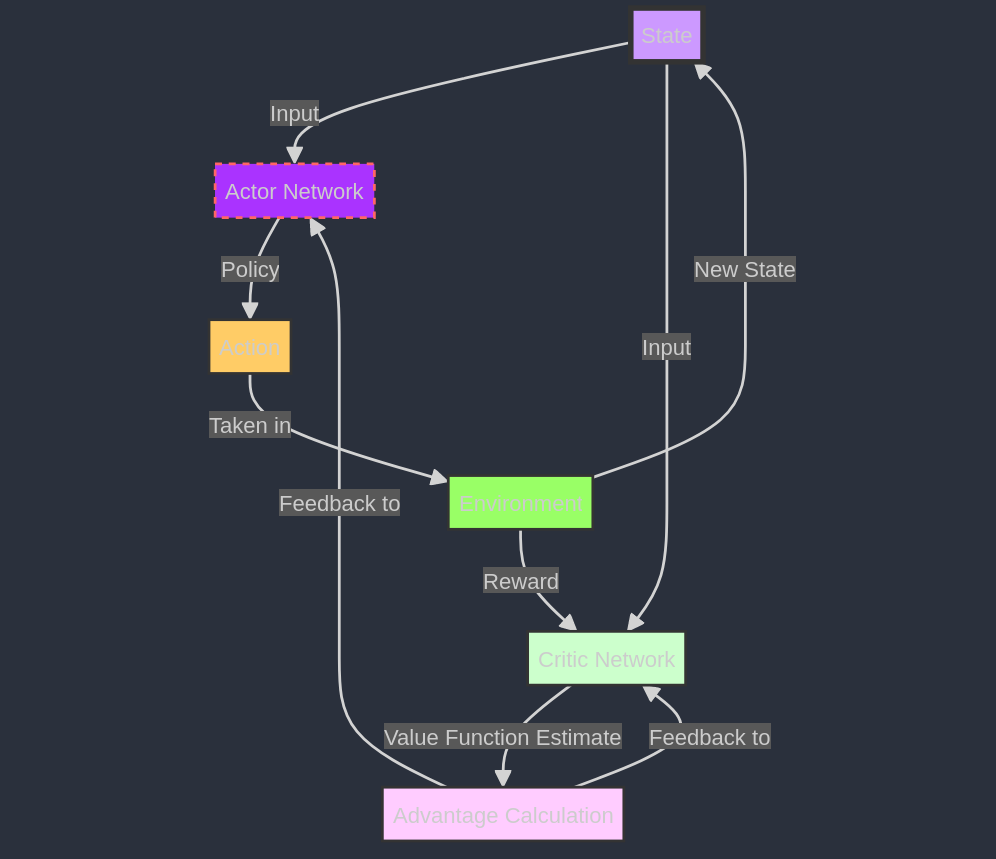
\includegraphics[width=0.5\textwidth]{Images/ppo_explanation.png}
    }
    \caption{Actor-Critic Method}\label{actor_critic}
\end{figure}

But the story doesn't end with PPO alone. Unity's ML-Agents toolkit, which is introduced in section$~$\ref{unity}, seamlessly integrates with PPO. ML-Agents provides a platform for training intelligent agents within the Unity environment, and when combined with the power of PPO, it paves the way for robust and efficient training regimes. This synergy between PPO and ML-Agents is particularly promising for complex simulations, such as kiteboat training, where agents can iteratively learn and refine their strategies for optimal performance$~$\cite{mlagents_ppo}.

The Proximal Policy Optimisation algorithm is a testament to the continuous evolution and innovation in the field of Reinforcement Learning. Its simplicity, efficiency, and robustness make it a prime choice for a huge range of applications. 

\section{Unity Game Engine}\label{unity}

Unity, a name that resonates with game developers was born in the city of Copenhagen, Denmark, in 2005, Unity has since evolved into a powerhouse, responsible for games like `Among Us' and `Pokemon Go' \cite{unity100seconds}.

At its heart, Unity is a cross-platform game engine designed to craft both 2D and 3D experiences. It offers a harmonious blend of a powerful graphical editor and the flexibility of \texttt{C\#} coding, allowing developers to translate their visions into virtual realities$~$\cite{unitymanual2021}, while the engine's core is written in C++.

Diving into the basics of Unity game development, one is greeted with a plethora of tools and components that simulate real-world interactions. Unity's lighting, physics, rigidbody, and colliders work in tandem to create immersive and impressively realistic environments. Whether it's the glint of sunlight reflecting off a surface or the bounce of a ball$~$\cite{goldstone2010}. Developers can further enhance objects with custom \texttt{C\#} scripts, giving rise to unique and custom gameplay experiences.

% Imagine crafting a game level: a dodgeball arena illuminated by a radiant light source, with a camera capturing every thrilling moment. Unity makes this possible with simple objects like planes, cylinders, and spheres. The intuitive interface allows developers to select, move, rotate, and scale objects with ease, setting the stage for an exhilarating match \cite{harrison2013}.

Unity's rigid body component adds a whole new dimension to game development, allowing them to be influenced by gravity. Combine this with the material component, and one can create mesmerising visual effects$~$\cite{blackman2012}. Unity has two types of gameplay updates: Update and FixedUpdate. While the former is called every frame during gameplay, ensuring fluid animations and interactions, the latter syncs with the physics engine's frame rate, making it ideal for moving objects around and applying forced in realtime$~$\cite{unityupdatefixedupdate}.

Unity's ML-Agents toolkit is a game-changer for those looking to infuse artificial intelligence into their games. ML-Agents provides a platform to train intelligent agents within the Unity environment using Reinforcement Learning, making it an ideal choice for complex simulations like kiteboat training. Unity is not just a game engine; it's a platform for innovation, and a testament to the limitless possibilities of virtual worlds.

\section{Existing Kiteboat Technologies}\label{sec:kiteboat_tech}
As kite technologies improve and kites become more mainstream and accessible, there are several companies that have started to explore the potential of kite-powered vessels, both for a commercial and recreational purpose. Wingit$~$\cite{wingit}, is a German company that have specialised in creating autonomous kite control systems that can be integrated onto pleasure vessels, seen earlier in figure$~$\ref{kiteboat}. This system can use any LEI (leading edge inflatable) kite and has its own custom kite-control-unit, as well as a remote control and autopilot. It is the autopilot that is particularly interesting, as this is what will be investigated throughout this thesis. The Wingit autopilot has 2 modes:
% \begin{figure}[!htb]
%     \centering
%     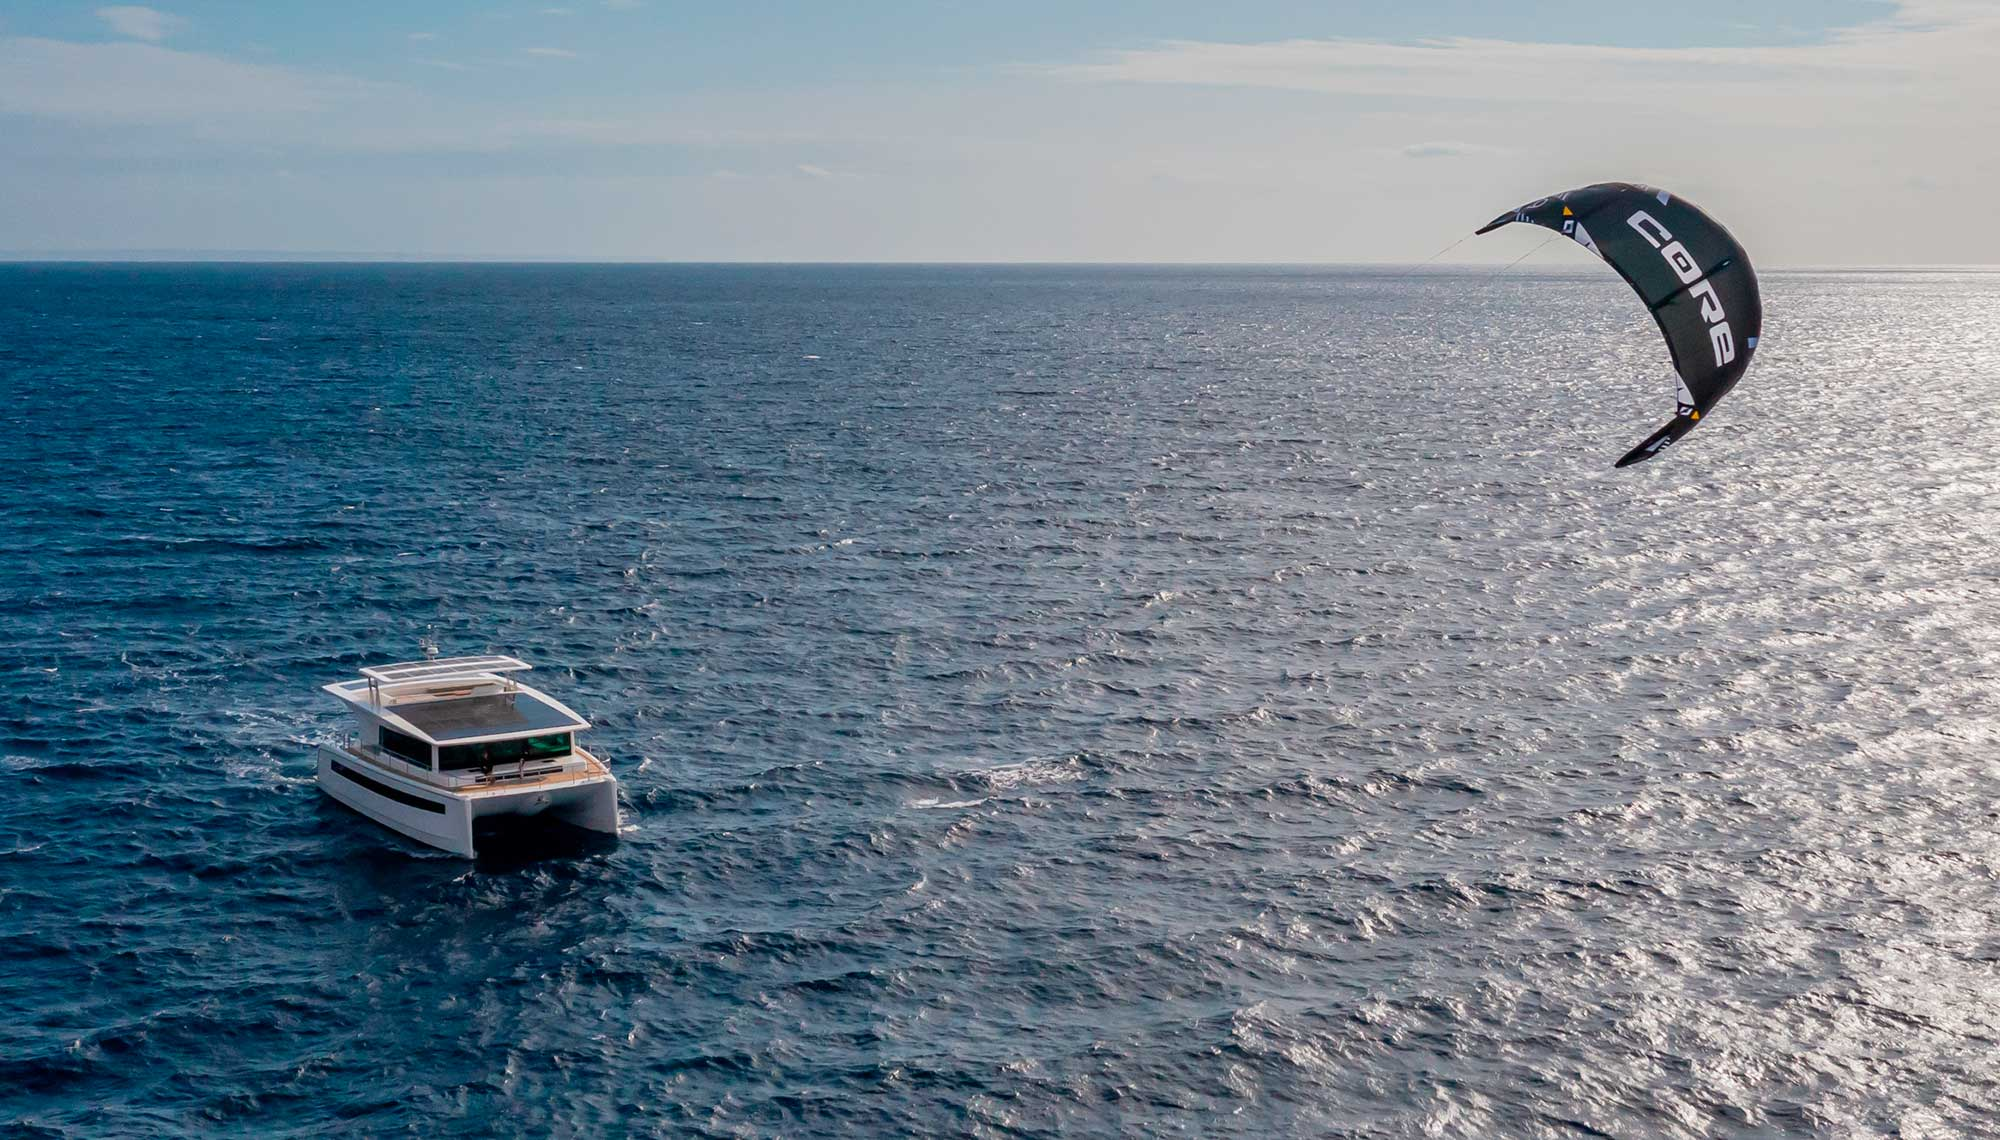
\includegraphics[width=0.8\textwidth]{Images/kiteboat.jpg}
%     \caption{Silent 60 with Wingit Kite Control}\label{kiteboat}
% \end{figure}
\begin{itemize}
    \item Lying Eight - The kite follows a horizontal figure of eight pattern, this is widely regarded as the best, most stable, and most consistent way to generate the maximum power.
    \item Zenith - The kite remains at 12 o'clock, directly above the boat.
\end{itemize}
The crucial thing about these modes is that they are pre-programmed. A complex control system, using line sensors to work out the position of the kite, has been created to allow the autopilot to fly the kite in these preconfigured patters and positions. This is at its core a PID controller, and while it is a good approach to controlling the kite, it is not very adaptable. 

Beyond The Sea$~$\cite{beyondthesea} is another company with kites as their primary focus. They are developing full solutions including kite and control systems for leisure and commercial applications. Their SeaKite seen in figure$~$\ref{seakite}, is their latest and most curring edge innovation, which claims to utilise some `AI' in its control mechanism. 

\begin{figure}
\centering
    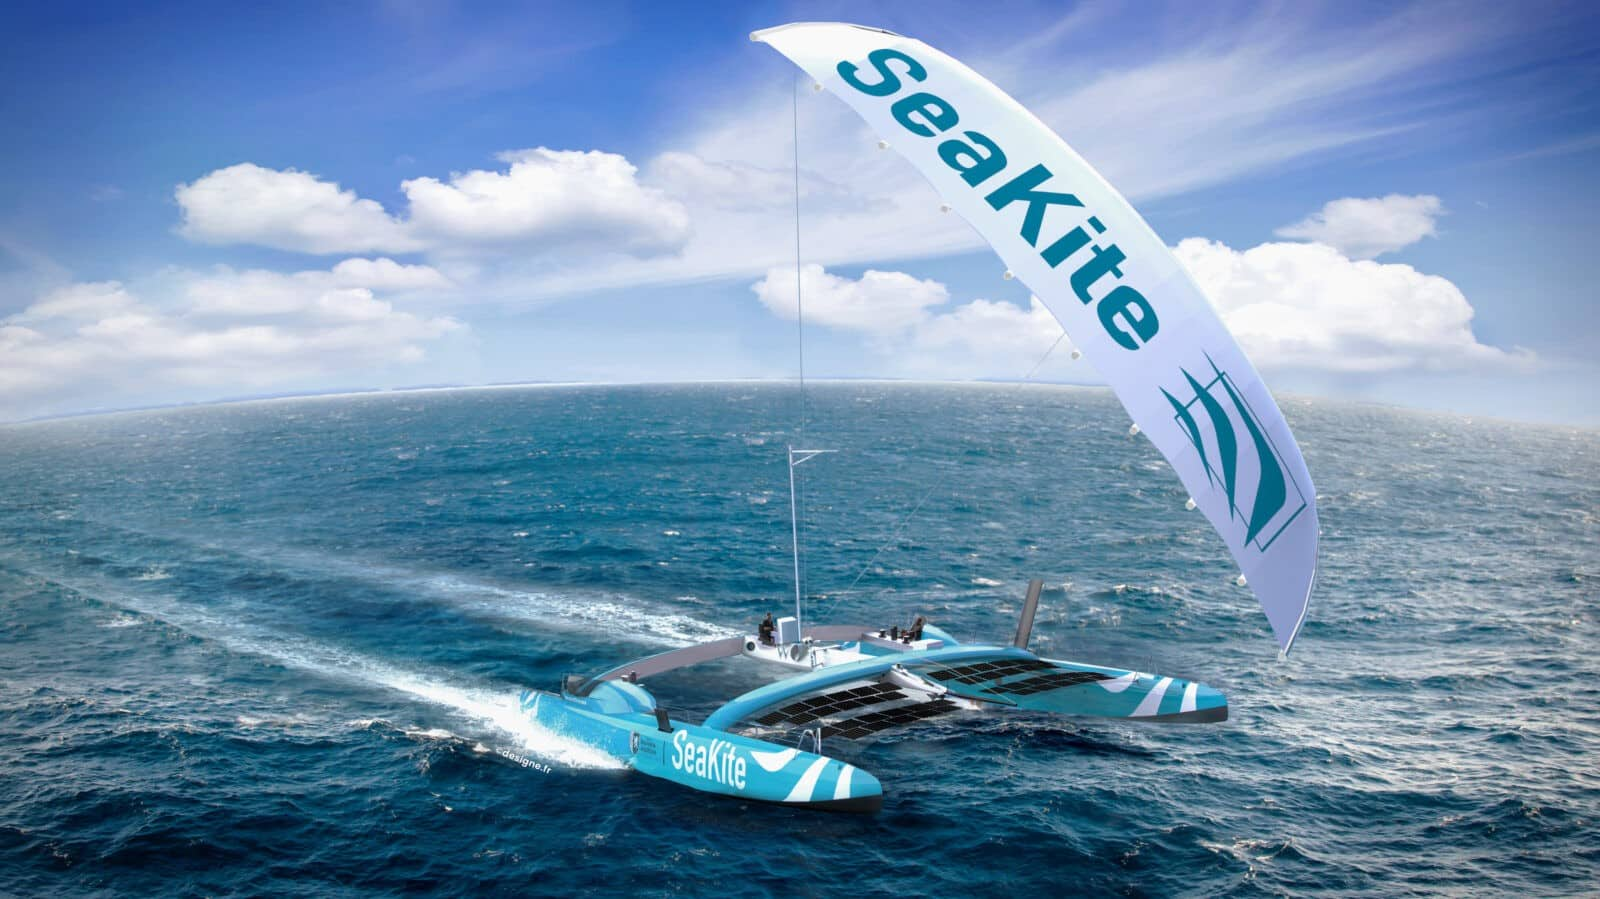
\includegraphics[width=0.8\textwidth]{Images/seakite.jpg}
    \caption{Beyond The Sea's `SeaKite'}\label{seakite}
\end{figure}

Autonomous control systems for kites are new of the last 10 years, but have primarily focused on methods utilised by Wingit, a pre-programmed control system. Due to the technological boom in artificial intelligence and computing in the last 5 years, forward thinking companies like Beyond The Sea are just starting to explore machine learning as an alternative control method. This project aims to do just that, explore the creation of an autonomous kite and boat control mechanism using machine learning.